\lecture{Tue. 9/25/12}

Let $M$ be a smooth manifold. %and $g$ be a Riemannian metric. 
We've looked at vector fields on $M$, $\X(M)$. We've also talked about
\begin{itemize}
\item
a connection $\nabla:\X(M)\times \X(M)\to \X(M)$, and
\item
a covariant derivative $\cvd$ along a curve.
\end{itemize}
{\it A priori}, this has nothing to do with geometric structure. 

We brought in the geometric structure using a Riemannian metric $g$. More generally, we can let $g$ be a symmetric nondegenerate bilinear form
\[
g:T_pM\times T_pM\to \R
\]
(smoothly varying in $p$).

Last time, we saw that given a smooth manifold and such a structure, we can define a compatible connection. 
%We can define parallel translation. 

The canonical example is $M=\R^n$, $g=\an{\cdot,\cdot}$, with $\an{(v_1,\ldots, v_n),(w_1,\ldots, w_n)}=v_iw_i$. The Levi-Civita connection is just taking the derivative of one vector-valued function in the direction of another.

Another example of particular interest is the following.
\begin{ex}[Minkowski space]
The space is $\R^n\times \R^{n+1}$, with coordinates $(x,t)$. The metric is given by
\[
\an{(v_1,\ldots, v_n,s_1),(w_1,\ldots, w_n,s_2)}_{\R^{n+1}}
=v_iw_i-s_1s_2.
\]
This is a nondegenerate symmetric bilinear form but it is not positive definite.

This is the canonical example of space-time.
\end{ex}
Keep in mind these examples.
\subsection{Geodesics}
%everything talked about so far work in examples of this nature.
If we take a curve $c$ and a vector field $V$ along $c$, then we can define a covariant derivative $\cvd V$. We said that $V$ is parallel if
\[
\cvd V=0.
\]
%all connections compatible
If we take vector fields $V_1$ and $V_2$, then
\[
\fc{d}{dt}\an{V_1,V_2}=\an{\cvd V_1,V_2}+\an{V_1,\cvd V_2}.
\]
\begin{df}
Let $c:I\to M$. Then $c'$ is a vector field along the curve. We say $c$ is a \textbf{geodesic} if $c'$ is a parallel vector field, i.e.
\[
\cvd c'=0.
\]
\end{df}
We now express numerically the condition for $c$ to be a geodesic.

\ig{6-1}{1}

Write the curve as $c(t)=(x_1(t),\ldots, x_n(t))$ in local coordinates.  Think of $c'(t)$ as on $TM$, which has coordinates $\pa{x_1,\ldots, x_n;y_1\pd{}{x_1},\ldots, y_n\pd{}{x_n}}$.
We have $c'(t)=(x_1(t),\ldots, x_n(t), x_1'(t),\ldots, x_n'(t))$, where $c'=x_j'\pd{}{x_j}$. Then
\beq{eq:965-6-1}
\cvd c'=\cvd  \pa{x_j'\pd{}{x_j}}=x_j''\pd{}{x_j}+x_j'\cvd \pd{}{x_j}.
\eeq
We can express $\pd{}{x_j}$ using the christoffel symbols
\beq{eq:965-6-2}
\cvd \pd{}{x_j}=\nabla_{c'}\pd{}{x_j}=x_i'\np{x_i}\pd{}{x_j}
=x_i'\Ga_{ij}^k\pd{}{x_k}.
\eeq
Substituting~\eqref{eq:965-6-2} with~\eqref{eq:965-6-1} gives
\begin{align*}
\cvd c'&=x_j''\pd{}{x_j}+x_j'x_i'\Ga_{ij}^k\pd{}{x_k}\\
&=x_j''\pd{}{x_j}+x_k'x_i'\Ga_{ik}^j\pd{}{x_j}\\
&=(x_j''+x_k'x_i'\Ga_{ik}^j)\pd{}{x_j}.
\end{align*}
The condition that $c$ is a geodesic is hence equivalent to
\beq{eq:965-6-3}
x_j''+x_i'x_k'\Ga_{ik}^j=0\text{ for all }j
\eeq
Supposing $c$ is a function on $I=[a,b]$, by the theory of ODE's, there is a unique solution given any choice of initial conditions
\[
x_i(a),\qquad x_i'(a),
\]
and we have smooth dependence on initial conditions. 
We have just proved the following.
\begin{thm}\llabel{thm:unique-geodesic}
Given a point $p\in M$ and a direction $v\in T_pM$, there is a unique geodesic $c$ starting at the point and going in that direction, i.e. with $c(0)=p$ and $c'(0)=v$.%%%%

Moreover, the curve depends smoothly on the initial conditions. 
\end{thm}
Because $c'$ is a geodesic we have
\[
\fc{d}{dt}g(c',c')=g(\cancelto{0}{\cvd c'},c')+g(c',\cancelto{0}{\cvd c'})=0
\]
%$t\to g(c',c')$ is consistent with the geodesic.

We give several easy observations. Let $c:[a,b]\to M$. 

\ig{diagrams/diags-1}{1}

Let $E_1,\ldots, E_n$ be a orthonormal basis at $T_{c(a)}M$. By parallel transport we get an orthonormal basis on every point of $c$; by abuse of notation we also denote them by $P_tE_i=E_i$. They remain orthonormal: $\fc{d}{dt}g(E_i,E_j)=\de_{ij}$. If $c$ is a geodesic with unit speed, i.e. $|c'|:=\sqrt{g(c',c')}=1$.

The following is elementary.
\begin{pr}\llabel{pr:geodesic-repar}
Suppose $c:[a,b]$ is a geodesic and $k$ is a constant. 
\begin{enumerate}
\item
Define the shifted curve $c_k(t)=c(t+k)$, $c_k:[a-k,b-k]\to M$.
\item
Define scaled curve $c^k(t)=c(kt)$, $c:\ba{\fc ak,\fc bk}\to M$.
\end{enumerate}
Then $c_k$ and $c^k$ are also geodesics.
\end{pr}
To keep our geodesic, we can't reparameterize by arbitrarily slowing down or speeding up, but we can shift the interval or go through the interval at a steady pace, but slower or faster.

\subsection{Exponential map}
\begin{df}
Given $p\in M$, define the \textbf{exponential map}\footnote{Note this is called the exponential map because for a Lie group, if we expand it out in Taylor series, it is just an exponential.} $\exp_p:T_pM\to M$ as follows. For $v\in T_pM$, let $c$ be the geodesic with $c(0)=p$ and $c'(0)=v$
\[
\exp_p(v)=c(1).
\]
\end{df}
This depends smoothly on the vector, by Theorem~\ref{thm:unique-geodesic} (which came from smoothness of ODE solutions in~\eqref{eq:965-6-3}).

\ig{diagrams/diags-4}{1}

Dropping the subscript, we think of $\exp$ as a map from the tangent bundle to $M$, $\exp:TM\to M$, such that if $(p,v)\in TM$ ($p\in M$, $v\in T_pM$), we have
\[
\exp((p,v))=\exp_pv.
\]
This is also smooth; we make use of the fact that the $x_i$ depend initially on both the initial conditions on the $x_i'$ and the $x_i$.

\subsubsection{Parameterized surface}
\begin{df}\llabel{df:psurf}
A \textbf{parameterized surface} is a smooth map
\[
F:[a,b]\times(-\ep,\ep)\to M.
\]
\end{df}
It may be an embedding, but this is not a requirement: it is allowed to map everything to a point.

\ig{diagrams/diags-2}{1}

Given a parameterized surface, we can look at two vector fields $\pd Fs$ and $\pd Ft$. 

\ig{diagrams/diags-3}{1}

\begin{pr}\llabel{pr:covar-commute}
We have the following:
\[
\cvd \pd{F}{s}=\fc{D}{\partial s}\pd{F}{t}.
\]
\end{pr}
Think of this as saying that ``derivatives commute."
\begin{proof}
Writing $F=(F_1,\ldots, F_n)$, we have
\begin{align*}
\pd{F}s&=\pd{F_i}s \pd{}{x_i}\\ 
\pd{F}t&=\pd{F_j}t \pd{}{x_j}\\
\cvd \pd Fs &=\cvd \pa{\pd{F_i}s\pd{}{x_i}}\\
&=\pd{^2F_i}{s\partial t}\pd{}{x_i}+\pd{F_i}{s}\cvd \pd{}{x_i}\\
&=\pd{^2F_i}{s\partial t}\pd{}{x_i}+\pd{F_i}{s}\nabla_{\pd{F_j}t\pd{}{x_j}} \pd{}{x_i}\\
&=\pd{^2F_i}{s\partial t}\pd{}{x_i}+\pd{F_j}t\pd{F_i}{s}\Ga_{ji}^k\pd{}{x_k}.
\end{align*}
This is symmetric in $s$ and $t$. The proposition follows.
\end{proof}



\subsubsection{Gauss Lemma}
We now make an observation about the exponential map. Usually we fix a point $p\in M$ and just think about $\exp_p:T_pM\to M$. We define by $\exp_p(v)=c(1)$ with $v\in T_pM$, $c(0)=p$ and $c'(0)=v$.

We can think of this another way. Recall that if we change the parameterization in a linear way, we still a geodesic (Proposition~\ref{pr:geodesic-repar}). 
%When $v=0$, the unique solution to $c(0)=p$, $c'(0)=0$ is the constant map, so $\exp_p(v)=p$.

%Now suppose $|v|\ne 0$, and let $w=\fc{v}{|v|}$. Let $c$ be the curve with $c(0)=p$ and $c'(0)=v$. Let $\ga$ be the geodesic with $\ga(0)=0$ and $\ga'(0)=w$. Then
%\[
%\exp_p(v)=c(1)=\ga(|v|).
%\]
%This is a direct consequence of reparametrization.
Now defining the geodesic $c$ such that $c(0)=p$ and $c'(0)=tv$, and letting $\ga$ be the geodesic with $\ga(0)=p$ and $\ga'(0)=v$, we have by reparameterization that $c(1)=\ga(t)$.
In other words, 
%From this we see that if $\ga$ is such that $\ga(0)=p$, and $\ga'(0)=v$.
\[
\exp_p(tv)= \ga(t).
\]
From this we see that {\it the exponential map sends lines in the tangent space at $p$ passing through 0 to geodesics passing through $p$ on the manifold}.\footnote{If you a  line or half-line in $T_pM$ starting  at some other point besides 0, then it may not get mapped to a geodesic.}

%We now use Proposition~\eqref{pr:covar-commute} to prove the Gauss lemma.

If $M$ were a two-dimensional, then $\exp_p:T_pM\to M$ is a parameterized surface. Furthermore, we could consider polar coordinates $(r,\te)$ on $T_pM$.  If the manifold is not 2-dimensional, restrict $\exp$ to a 2-dimensional subspace of $T_pM$, $\exp:V\to M$.

In either case we have a parameterized surface. 
\begin{lem}\llabel{lem:gauss}
Let $M$ be a manifold and $p\in M$. Let $\exp_p:T_pM\to M$. Let $V$ be a 2-dimensional subspace of $T_pM$, expressed in polar coordinates, and consider $\exp_p:V\to M$ as a function of $r$ and $\te$. Then
\[
g\pa{\pd{}{r}\exp_p,\pd{}{\te} \exp_p}=0.
\]
\end{lem}
%rays are mapped to geodesics
%The exponential map is just starting out from $p$ going in direction $v$.
In other words, the images of the circles in the tangent space are orthogonal to the geodesics starting at $p$.

\begin{center}
\begin{minipage}[c]{3 in}
\includegraphics{diagrams/diags-5}
\end{minipage}
$\Huge\rightarrow$
\begin{minipage}[c]{3 in}
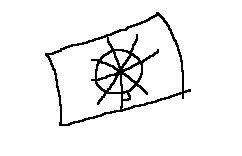
\includegraphics{6-2}
\end{minipage}
\end{center}

\begin{proof}
We can think of $g\pa{\pd{}{r}\exp_p,\pd{}{\te} \exp_p}$ as a function of $r$ and $\te$. We have, because $\exp_p(rv)$ is a geodesic for any $v$, that
\bal
\fc{d}{dr}g\pa{\pd{}{r}\exp_p,\pd{}{\te} \exp_p}
&=g\Big(\cancelto{0}{\fc{D}{\pl r} \pd{}{r}\exp_p}, \pd{}{\te}\exp_p\Big)+g\pa{\pd{}{r}\exp_p,\fc{D}{\pl r} \pd{}{\te}\exp_p}.\\
&=g\pa{
\pd{}{r}\exp_p,\frac{D}{\partial \te}\pd{}{r}\exp_p
}&\text{ by Proposition~\ref{pr:covar-commute}}\\
&=\rc2\pd{}{\te} g\pa{\pd{}{r}\exp_p,\pd{}{r}\exp_p}=0
\end{align*}
where the last equality follows from the fact that the velocity vector for a geodesic always has the same length. 
Hence $g\pa{\pd{}{r}\exp_p,\pd{}{\te} \exp_p}$ is constant. We just need to evaluate at origin, but it is clearly 0 at the origin.
\end{proof}
Next time we'll use the Gauss lemma to show geodesics are locally the shortest route.